\documentclass[addpoints]{exam}

\usepackage{amsmath}
\usepackage{amssymb}
\usepackage{graphicx}
\usepackage{hyperref}
\usepackage{multicol}
\usepackage{tikz}
\usepackage{titling}

% Header and footer.
\pagestyle{headandfoot}
\runningheadrule
\runningfootrule
\runningheader{CS 113 Spring 201}{HW 3: Inference and Relations}{\theauthor}
\runningfooter{}{Page \thepage\ of \numpages}{}
\firstpageheader{}{}{}

\boxedpoints
\printanswers

\newcommand\union\cup
\newcommand\interx\cap

\title{Homework 3: Inference and Relations\\ CS 113 Discrete Mathematics\\ Habib University -- Spring 2021}
\author{Don't Grade Me}  % replace with your ID, e.g. oy02945
\date{}

\begin{document}
\maketitle

\begin{questions}

  \section{Inference}

\question This question refers to the \textit{tiling} or \href{https://en.wikipedia.org/wiki/Tessellation}{\textit{tessellation}} operation.
  
  \begin{minipage}{0.5 \linewidth}
    Given a standard checkerboard and dominoes, answer the following questions. Explain your answer for each question.\\
    \begin{center}
      \includegraphics[width= 0.15\textwidth]{dominos}
    \end{center}
  \end{minipage} 
  \begin{minipage}{0.5 \linewidth}\begin{center}
      \includegraphics[width=0.6 \textwidth]{checkerboard} \end{center}
  \end{minipage}
  \begin{parts}
  \part[5] Can we tile the standard checkerboard using dominoes?
    \begin{solution}
      % Write your solution here
    \end{solution}
    
  \part[5] Can we tile a checkerboard obtained by removing one of the four corner squares of a standard checkerboard?
    \begin{solution}
      % Write your solution here
    \end{solution}
    
  \part[5] Can we tile a board obtained by removing both the upper left and the lower right squares of a standard checkerboard? 
    \begin{solution}
      % Write your solution here
    \end{solution}
  \end{parts}

\question[10]
  The following is a murder case solved by Sherlock Holmes, in “A Study
  in Scarlet” :\\
  \textit{“And now we come to the great question as to the reason why. Robbery
    has not been the object of the murder, for nothing was taken. Was it
    politics, then, or was it a woman?  That is the question which confronted
    me. I was inclined from the first to the latter supposition. Political
    assassins are only too glad to do their work and fly. This murder had, on
    the contrary, been done most deliberately, and the perpetrator has left
    his tracks all over the room, showing he had been
    there all the time.”}\\
  From these, Sherlock Holmes concluded: ``It was a woman''.  Translate the
  above argument to statements in predicate logic and prove its validity.
  \begin{solution}
    % Write your solution here
  \end{solution}

  
\question Prove the following arguments using inference rules. Mention the rule(s) that you use at each step.
  \begin{parts}
    
  \part[5] $ $\\
    \begin{tabular}{ll}
      P1 &  If it is Sunday today, then we play cricket or basketball.\\
      P2 &  If the basketball field is occupied, we don't play basketball.\\
      P3 &  It is Sunday today, and the basketball field is occupied.    \\
      \hline
      C & We play cricket or volleyball. 
    \end{tabular}
    \begin{solution}
      \\ Q is we play cricket \\ V is we play Volleyball \\ R is we play Basketball \\ F is the Field is occupied \\ P is It is Sunday today \\ We need to prove Q  $ \lor$ V \\ P1: P $\implies$ (Q $\lor$ R) \\ Premise P \\ Applying Modus Ponens to these premises gives us Q  $ \lor$ R \\ P2: S $\implies$ $\neg$ R \\ Applying Modus Ponens gives us $\neg$ R \\ Applying Disjunctive Syllogism to Q  $ \lor$ V and $\neg$ R giving us the result Q \\ Applying Addition rule on Q to get  Q  $ \lor$ V
    \end{solution}
    
  \part[10]  $ $\\
    \begin{tabular}{ll}
      P1 &  Ahmed failed the course, but attended every lecture. \\
      P2 &  Everyone who did the homework every week passed the course. \\
      P3 &  If a student passed the course, then they did some of the homework.\\
      \hline
      C & Not every student did every homework assignment.
    \end{tabular}

    \begin{solution}
      % Write your solution here
    \end{solution}
  \end{parts}


\question[5]
  Consider the statement: The remainder of the square of any odd number when divided by 4 is 1.
  
  \begin{parts}
  \part[5] Write the above statement using predicate logic notation and prove it.
    \begin{solution} 
      % Write your solution here
    \end{solution}
    
  \part[5] Prove whether the statement holds even when written as a bi-conditional.
    \begin{solution}
      % Write your solution here
    \end{solution}
  \end{parts}

\question[5]
  Show that these statements about the real number $x$ are equivalent: (i) x is irrational, (ii)  $\frac{x}{2}$ is irrational. Which proof method did you use?

  \begin{solution}
    % Write your solution here
  \end{solution}
  
  \section{Equivalence Relation}
  
\question Prove or disprove whether each of the relations represented below is an equivalence relation.
    \begin{parts}
    \part[5] $R \text{ on } \mathbb{R} = \{ (x,y) \mid xy\geq 0\}$
    \part[5] $R \text{ on } \mathbb{R} = \{ (x,y) \mid x = 1\}$
    \part[5] $\begin{bmatrix} 1 & 0 & 1 & 0 \\ 0 & 1 & 0 & 1 \\1 & 0 & 1 & 0 \\ 0 & 1 & 0 & 1 \end{bmatrix}$
    \part[5] $\begin{bmatrix} 1 & 1 & 1 & 0 \\ 1 & 1 & 1 & 0 \\ 1 & 1 & 1 & 0 \\ 0 & 0 & 0 & 1 \end{bmatrix}$
    \part[5] $R_1 \interx R_2$ where $R_1$ and $R_2$ are equivalence relations on a set, $S$.
    \end{parts}
  \begin{solution}
    % Write your solutions here
    \begin{parts}
    \part
    The relation given is not an equivalence relation as it is not transitive. Assuming (x,y,z) to be (-3,0,1) then yz $\geq 0$, xy $\geq 0$ but not for xz as -3 is less than 0 
    \part
    It is not symmetric and hence does not an equivalence relation
    \part
    symmetric as Tij=1 and Tji=1 and same for 0 as well.\\ Reflexive as all diagonals have value 1 \\ Transitive as multiplying the matrix by itself gives us:\\ T = $\begin{bmatrix} 2 & 0 & 2 & 0 \\ 0 & 2 & 0 & 2 \\2 & 0 & 2 & 0 \\ 0 & 2 & 0 & 2 \end{bmatrix}$
    \part
    Reflexive as all diagonals have value 1 \\ symmetric as Tij=1 and Tji=1 and same for 0 as well \\ Transitive as multiplying the matrix by itself gives us:\\  T = $\begin{bmatrix} 3 & 3 & 3 & 0 \\ 3 & 3 & 3 & 0 \\ 3 & 3 & 3 & 0 \\ 0 & 0 & 0 & 3 \end{bmatrix}$
    \part
    \end{parts}    
  \end{solution}

  \begin{EnvUplevel}
    Let $R$ be a relation from a set A to a set B. The \textit{inverse relation} from $B$ to $A$, denoted by $R^{-1}$, is the set of ordered pairs $\{(b, a) \mid (a, b) \in R\}$. The \textit{complementary relation} $\overline{R}$ is the set of ordered pairs $\{(a, b) \mid (a, b) \not\in R\}$. A relation $R$ on the set $A$ is \textit{irreflexive} if $\forall a \in A\colon (a, a) \not\in R$. That is, $R$ is irreflexive if no element in $A$ is related to itself.
  \end{EnvUplevel}

\question 
  \begin{parts}
  \part[5] Show that the relation $R$ on a set $A$ is symmetric if and only if $R = R^{-1}$.
    \begin{solution}
      % Write your solution here
    \end{solution}

  \part[5] Show that the relation $R$ on a set $A$ is reflexive if and only if $\overline{R}$ is irreflexive.
    \begin{solution}
      % Write your solution here
    \end{solution}

  \part[5] Let $R$ be a relation that is reflexive and transitive. Prove that $R^n = R$ for all positive integers $n$.
    \begin{solution}
      % Write your solution here
    \end{solution}

  \part[5] Show that the relation $R$ on a set $A$ is transitive if and only if $R^n \subseteq R$ for all positive integers $n$.
    \begin{solution}
      % Write your solution here
    \end{solution}

  \end{parts}
  
\question  Given the matrix, $M_R$, for a relation, $R$, on a finite set, $A$, explain how to obtain the following matrices?
  \begin{multicols}{2}
    \begin{parts}
    \part[5] $M_{R^{-1}}$
    \part[5] $M_{\overline{R}}$
    \end{parts}
  \end{multicols}
  \begin{solution}
    % Write your solutions here
    \begin{parts}
    \part 
    \part 
    \end{parts}
  \end{solution}
  
\question The following questions refer to the relations, $R$ and $S$, involving the set $X = \{a, b, c\}$. Specifically, $R$ and $S$ are relations on $2^X$, the power set of $X$. For the definitions of $R$ and $S$ given below, prove whether each is an equivalence relation.
  \begin{multicols}{2}
    \begin{parts}
    \part[5] $R = \{(A, B) \mid |A| = |B|\}$.
    \part[5] $S = \{(A, B) \mid |A| < |B|\}$.
    \end{parts}
  \end{multicols}
  \begin{solution}
    % Write your solutions here
    \begin{parts}
    \part 
    \part 
    \end{parts}
  \end{solution}

\question[5] A partition $P_1$ is called a \textit{refinement} of the partition $P_2$ if every set in $P_1$ is a subset of one of the sets in $P_2$. Given equivalence relations, $R_1$ and $R_2$, on a set, $A$, and the corresponding partitions, $P_1$ and $P_2$, show that $R_1 \subseteq R_2$ if and only if $P_1$ is a refinement of $P_2$.
  \begin{solution}
    % Write your solution here
  \end{solution}

\section{Ordering}
  
\question Prove or disprove whether each of the relations represented below is a partial order.
  \begin{multicols}{3}
    \begin{parts}
    \part[5] $\begin{bmatrix} 1 & 1 & 1 \\ 1 & 1 & 0 \\ 0 & 0 & 1 \end{bmatrix}$
    \part[5] $\begin{bmatrix} 1 & 1 & 1 & 0 \\ 1 & 1 & 1 & 0 \\ 0 & 0 & 1 & 1 \\ 1 & 1 & 0 & 1 \end{bmatrix}$
    \end{parts}
  \end{multicols}
  \begin{solution}
    % Write your solutions here
    \begin{parts}
    \part 
    \part 
    \end{parts}
  \end{solution}
  
\question[5] Given a poset $(S, R)$, its \textit{dual} is $(S,R^{-1})$. Show that the dual is also a poset. 
  \begin{solution}
    % Write your solution here    
  \end{solution}
  
\question Answer the following questions for the partial order represented by the given Hasse diagram.
  
  \begin{minipage}{.3\textwidth}
    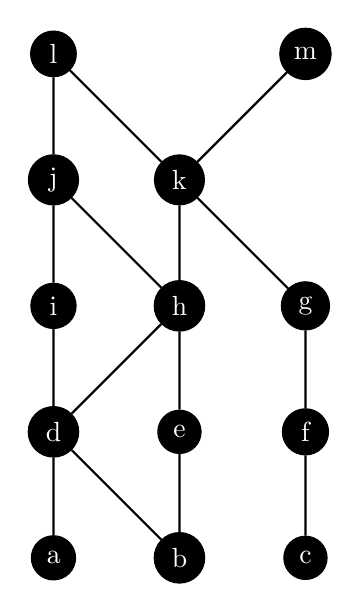
\begin{tikzpicture}[scale=0.8]
      \tikzstyle{node} = [draw,circle,fill=black,text=white]

      \def\nodes{a,b,c,d,e,f,i,h,g,j,k}
      \foreach \n/\p
      [count=\i from 0,
      evaluate= \i as \x using {2*Mod(\i,3)},
      evaluate= \i as \y using {2*int(\i/3)}]
      in \nodes {
        \node[node](\n) at (\x,\y) {\n};
      }
      \node[node](l) at (0,8) {l};
      \node[node](m) at (4,8) {m};

      \draw[thick,-] (a) -- (d) -- (i) -- (j) -- (h) -- (d) -- (b) -- (e) -- (h) -- (k) -- (l) -- (j);
      \draw[thick,-] (c) -- (f) -- (g) -- (k) -- (m);
      
    \end{tikzpicture}
  \end{minipage}
  \begin{minipage}{.65\textwidth}
    \begin{parts}
    \part[2] Find the maximal elements.
    \part[2] Find the minimal elements.
    \part[1] Is there a greatest element? If so, what is it?
    \part[1] Is there a least element? If so, what is it?
    \part[2] Find all upper bounds of $\{a,b,c\}$.
    \part[1] Find the least upper bound of $\{a,b,c\}$, if it exists.
    \part[2] Find all lower bounds of $\{f,g,h\}$.
    \part[1] Find the greatest lower bound of $\{f,g,h\}$, if it exists.
    \end{parts}
  \end{minipage}
  \begin{solution}
    % Write your solutions here
    \begin{parts}
    \part 
    \part 
    \part 
    \part 
    \part 
    \part 
    \part 
    \part 
    \end{parts}
  \end{solution}

  
\end{questions}

\end{document}


%%% Local Variables:
%%% mode: latex
%%% TeX-master: t
%%% End:
